\chapter{HASIL PREPROCESSING}
\label{chap:prepro}

Bab ini memuat jenis publikasi pada \textit{dump}, hasil tiap tahap \textit{preprocessing}, dan statistik \textit{dataset} bersih (\textit{Task} 1).

\section{Jenis publikasi}
\label{sec:hasil-jenis}
Tabel~\ref{tab:jenis} menunjukkan jumlah \textit{record} per jenis publikasi pada seluruh \textit{dump} dan pada periode 2015--2025, dan Gambar~\ref{fig:jenis} menggambarkannya pada skala logaritmik.

\begin{table}[ht]
\caption{Jumlah \textit{record} per jenis publikasi DBLP}
\label{tab:jenis}
\small
\begin{tabularx}{\textwidth}{@{}p{3.2cm}>{\raggedright\arraybackslash}X rrr@{}}
\toprule
\textbf{Jenis} & \textbf{Arti} & \textbf{Seluruh DBLP} & \textbf{2015--2025} & \textbf{Porsi} \\
\midrule
\texttt{article} & Artikel jurnal & 4.527.388 & 2.735.633 & 60,4\% \\
\texttt{www} & Halaman profil penulis & 4.247.510 & 1 & 0,0\% \\
\texttt{inproceedings} & Makalah konferensi dan \textit{workshop} & 4.004.309 & 2.004.202 & 50,1\% \\
\texttt{phdthesis} & Disertasi & 158.395 & 71.290 & 45,0\% \\
\texttt{incollection} & Bab dalam buku & 71.264 & 21.625 & 30,3\% \\
\texttt{proceedings} & Buku prosiding induk & 65.903 & 31.809 & 48,3\% \\
\texttt{data} & \textit{Dataset} & 31.529 & 22.230 & 70,5\% \\
\texttt{book} & Buku & 21.654 & 5.813 & 26,8\% \\
\texttt{mastersthesis} & Tesis magister & 27 & 4 & 14,8\% \\
\midrule
\textbf{Total} & & \textbf{13.127.979} & & \\
\bottomrule
\end{tabularx}
\end{table}

\begin{figure}[ht]
\centering
\figtikz{fig-jenis-publikasi}
\caption{Jumlah \textit{record} per jenis publikasi, seluruh \textit{dump} dibandingkan dengan periode 2015--2025 (skala logaritmik)}
\label{fig:jenis}
\end{figure}

Jenis \texttt{article} dan \texttt{www} menyumbang sekitar 67\% isi \textit{dump}, sedangkan \texttt{inproceedings} hanya 30,5\%. Separuh \texttt{inproceedings} (50,1\%) terbit pada 2015--2025. Jenis \texttt{www} hanya memiliki satu \textit{record} pada periode ini karena itu adalah halaman profil penulis yang umumnya tidak bertahun. Jenis \texttt{proceedings} adalah buku prosiding induk yang dirujuk lewat \texttt{crossref}, bukan makalah.

\section{Hasil preprocessing}
\label{sec:hasil-prepro}
Data berkurang dari 2.004.202 menjadi 1.997.244 makalah, yaitu 6.958 makalah (0,35\%) dibuang dan 99,65\% dipertahankan. Tabel~\ref{tab:dampak} merinci dampak tiap tahap dan Gambar~\ref{fig:alur-seleksi} memperlihatkan alurnya dari seluruh \textit{dump}.

\begin{table}[ht]
\caption{Dampak tiap tahap \textit{preprocessing}}
\label{tab:dampak}
\small
\begin{tabularx}{\textwidth}{@{}>{\raggedright\arraybackslash}X rrr@{}}
\toprule
\textbf{Tahap} & \textbf{Dibuang} & \textbf{Tersisa} & \textbf{Porsi dibuang} \\
\midrule
0. Data mentah (\texttt{inproceedings} 2015--2025) & & 2.004.202 & \\
1. Konsistensi tahun & 0 & 2.004.202 & 0\% \\
2. Makalah tanpa penulis & 2.255 & 2.001.947 & 32\% \\
3. \textit{Key} bukan \texttt{conf/} & 3.161 & 1.998.786 & 45\% \\
4. Duplikat judul, tahun, dan \textit{venue} & 1.542 & 1.997.244 & 22\% \\
5. Normalisasi penulis & 0 & 1.997.244 & 0\% \\
\midrule
\textbf{Total} & \textbf{6.958} & \textbf{1.997.244} & \textbf{100\%} \\
\bottomrule
\end{tabularx}
\end{table}

\begin{figure}[ht]
\centering
\figtikz{fig-alur-seleksi}
\caption{Alur seleksi data dari seluruh \textit{dump} sampai \textit{dataset} bersih}
\label{fig:alur-seleksi}
\end{figure}

Hasil setiap tahap diuraikan berikut ini.

\textbf{Konsistensi tahun.} Seluruh nilai \texttt{year} berupa empat digit dan berada pada 2015--2025 sehingga tidak ada baris yang dibuang. Penyaringan rentang sebenarnya sudah dilakukan saat ekstraksi sehingga tahap ini berfungsi sebagai validasi dan konversi tipe.

\textbf{Missing values.} Makalah tanpa penulis dibuang (2.255 makalah) karena tidak dapat masuk transaksi, dan isinya hampir seluruhnya halaman depan prosiding. Kolom \textit{booktitle} (190 kosong) dan \textit{crossref} (2.471 kosong) dibiarkan karena tidak dipakai, sedangkan \textit{title} dan \textit{year} tidak ada yang kosong.

\textbf{Normalisasi venue.} Seleksi \texttt{conf/} membuang 3.161 makalah, dan penurunan \textit{venue} dari \textit{key} mengubah 8.784 nama \textit{booktitle} menjadi 4.373 \textit{venue}. Sebanyak 1.270 \textit{venue} (29,0\%) memiliki lebih dari satu variasi \textit{booktitle}, dan 377.262 makalah (18,9\%) memakai \textit{booktitle} yang bukan nama dominan \textit{venue}-nya.

\textbf{Duplikat.} Terdapat 1.373 grup makalah dengan judul, tahun, dan \textit{venue} yang sama sehingga 1.542 baris dibuang (0,08\%). Seluruh anggota grup memiliki \textit{key} berbeda, biasanya dengan akhiran huruf (\texttt{...23} dan \texttt{...23a}). Tabel~\ref{tab:duplikat} menunjukkan bahwa sekitar 80\% grup memiliki daftar penulis yang identik sehingga hampir pasti duplikat. Sisanya berupa campuran: makalah sama dengan urutan penulis berbeda, ejaan nama berbeda (\textit{Joaquin} dan \textit{Joaquín}), himpunan bagian penulis, dan judul generik seperti \textit{Preface} (27 grup).

\begin{table}[ht]
\caption{Rincian grup duplikat}
\label{tab:duplikat}
\small
\begin{tabular}{@{}lrr@{}}
\toprule
\textbf{Jenis grup} & \textbf{Grup} & \textbf{Baris dibuang} \\
\midrule
Daftar penulis identik & 1.100 (80,1\%) & 1.121 \\
Daftar penulis berbeda & 273 (19,9\%) & 421 \\
\bottomrule
\end{tabular}
\end{table}

\textbf{Normalisasi penulis.} Normalisasi NFKC dan perapian spasi \textbf{tidak mengubah satu pun} dari 7.870.999 kemunculan nama, dan jumlah nama unik tetap 1.821.757 sebelum dan sesudahnya. DBLP sudah menyajikan nama dalam bentuk yang bersih sehingga tahap ini berfungsi sebagai pengaman. Beberapa temuan lain dicatat.
\begin{enumerate}
\item Sebanyak 97 pasangan makalah-penulis ganda dalam satu makalah dibuang (7.870.999 menjadi 7.870.902).
\item Sebanyak 90.593 nama membawa sufiks disambiguasi DBLP (\textit{Wei Wang 0001}) dan dipertahankan karena menghapusnya menggabungkan orang berbeda.
\item Sebanyak 7.573 kelompok nama (0,42\% dari nama unik) hanya berbeda huruf besar-kecil atau diakritik (\textit{A. Gómez} dan \textit{A. Gomez}). Kelompok ini tidak digabung karena sebagian besar berupa inisial yang sudah ambigu.
\item Masalah sebaliknya lebih berpengaruh: nama umum tanpa sufiks mewakili banyak orang. \textit{Yang Liu} tercatat pada 332 \textit{venue} dan 725 makalah, dan \textit{Wei Wang} pada 280 \textit{venue}.
\end{enumerate}

\section{Statistik dataset bersih}
\label{sec:hasil-statistik}
Tabel~\ref{tab:statistik} merangkum statistik \textit{dataset} setelah \textit{preprocessing}. Seluruh angka dihitung dari tabel Parquet hasil \textit{preprocessing}. Pasangan makalah-penulis hampir empat kali jumlah makalah karena satu makalah memiliki beberapa penulis.

\begin{table}[ht]
\caption{Statistik \textit{dataset} setelah \textit{preprocessing}}
\label{tab:statistik}
\begin{tabular}{@{}lr@{}}
\toprule
\textbf{Statistik} & \textbf{Nilai} \\
\midrule
Total publikasi & 1.997.244 \\
Total penulis unik & 1.821.757 \\
Total konferensi atau \textit{venue} unik & 4.373 \\
Pasangan makalah-penulis & 7.870.902 \\
Penulis per makalah (median dan rata-rata) & 4 dan 3,94 \\
Makalah per penulis (median dan rata-rata) & 1 dan 4,32 \\
Penulis dengan satu makalah & 51,4\% \\
\bottomrule
\end{tabular}
\end{table}

\subsection{Distribusi per tahun}
\label{sec:hasil-tahun}
Gambar~\ref{fig:per-tahun} menunjukkan jumlah publikasi per tahun. Jumlah publikasi naik dari 160.800 pada 2015 ke puncak 213.328 pada 2024, yaitu kenaikan 32,7\% atau CAGR 3,2\% per tahun. Garis tren linear menambah rata-rata 4.796 makalah per tahun. Pada 2020, jumlah turun 8,8\% dan tetap di bawah garis tren sampai 2022, lalu kembali di atasnya pada 2023 (naik 13,1\%). Kaitan penurunan ini dengan pandemi hanya dugaan karena data tidak memuat penyebabnya.

\begin{figure}[ht]
\centering
\figtikz{fig-publikasi-tahun}
\caption{Jumlah publikasi per tahun, 2015--2025}
\label{fig:per-tahun}
\end{figure}

\label{sec:hasil-2025}
Penurunan 6,5\% pada 2025 bukan penurunan aktivitas. Sebanyak 789 konferensi aktif pada 2024 tetapi kosong pada 2025, dan konferensi tersebut menyumbang 49.328 makalah (23,1\% dari total 2024). Ada dua penyebab yang berbeda, terlihat dari pola tahunannya.
\begin{enumerate}
\item Konferensi dua tahunan genap, seperti ECCV (1.638 makalah pada 2020, 0 pada 2021, 2.011 pada 2022, 0 pada 2023, 2.957 pada 2024, dan 0 pada 2025) dan ICPR, memang tidak diadakan pada 2025.
\item Konferensi tahunan yang prosidingnya belum terindeks, seperti IGARSS (2.589 makalah pada 2024), ICCCNT (2.119), dan EMBC (1.386), memiliki data setiap tahun sampai 2024 lalu kosong pada 2025.
\end{enumerate}
Sebaliknya, 322 konferensi kosong pada 2024 tetapi aktif pada 2025 (17.785 makalah), umumnya konferensi dua tahunan ganjil. Jika 789 konferensi yang kosong dikeluarkan, jumlah makalah 2025 berada 21,7\% di atas 2024. Angka ini bukan ukuran pertumbuhan yang adil karena 322 konferensi yang hanya aktif pada 2025 tetap terhitung. Meskipun demikian, angka tersebut cukup untuk menunjukkan bahwa penurunan 6,5\% adalah efek komposisi. Karena itu 2025 digambar dengan arsiran dan tidak dipakai menghitung CAGR maupun garis tren.

\subsection{Distribusi per konferensi}
\label{sec:hasil-konferensi}
Sepuluh konferensi teratas menghasilkan 9,4\% publikasi dan dua puluh teratas 15,6\%. Sebanyak 231 dari 4.373 \textit{venue} (5,3\%) menghasilkan separuh publikasi, dan 1.011 \textit{venue} (23,1\%) menghasilkan 80\%. Median \textit{venue} hanya memiliki 134 makalah selama sebelas tahun, dengan rata-rata 457 dan maksimum 25.455 (NeurIPS). Sebanyak 1.358 \textit{venue} (31,1\%) memiliki kurang dari 50 makalah. Distribusi ini sangat condong ke kanan: sedikit konferensi sangat besar dan banyak konferensi kecil (Gambar~\ref{fig:ukuran-venue}). Sepuluh konferensi terbesar dibahas pada Subbab~\ref{sec:hasil-t2}.

\begin{figure}[ht]
\centering
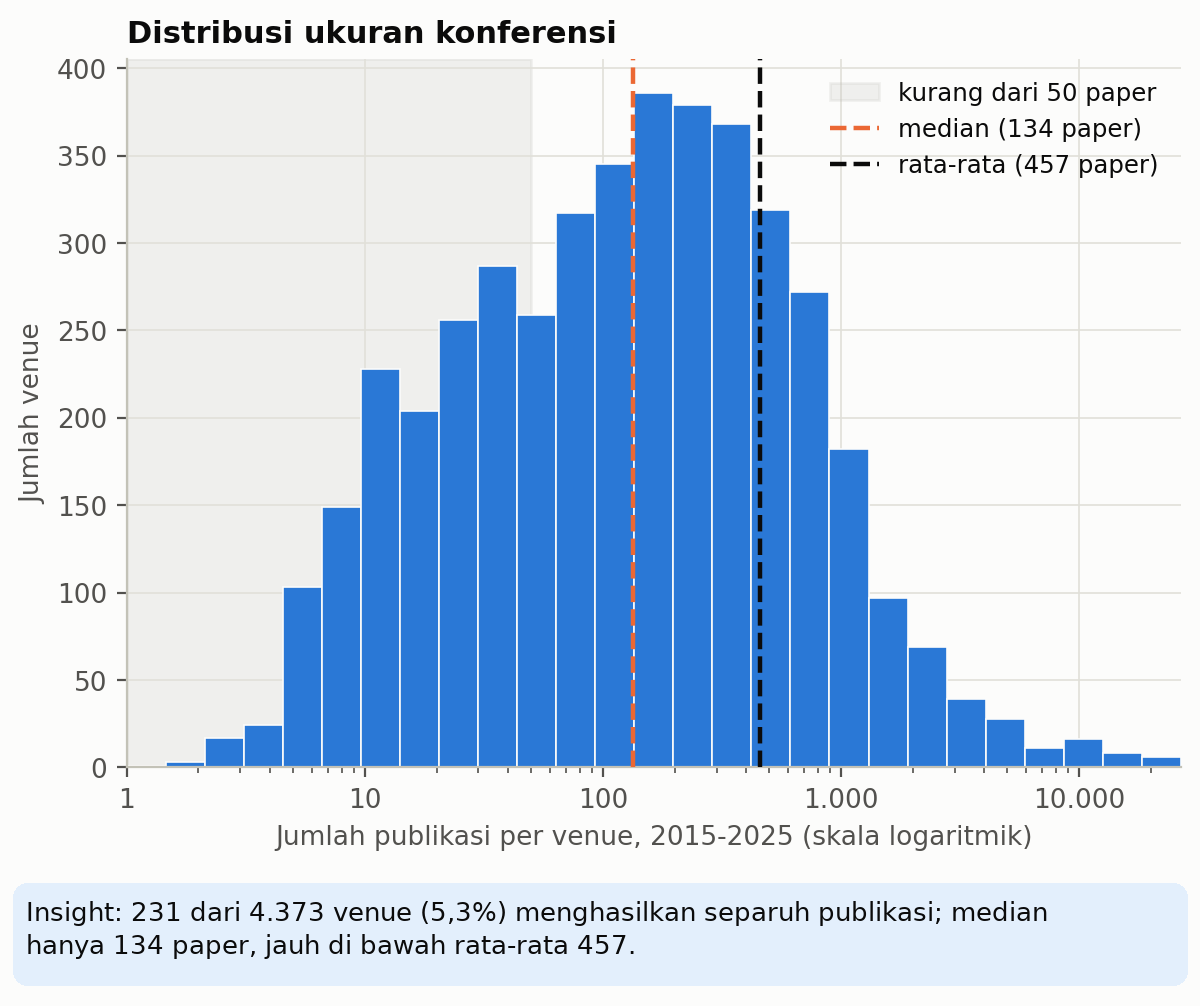
\includegraphics[width=\textwidth]{images/hasil/t1_distribusi_ukuran_venue.png}
\caption{Distribusi ukuran \textit{venue} berdasarkan jumlah makalah}
\label{fig:ukuran-venue}
\end{figure}

\subsection{Distribusi penulis}
\label{sec:hasil-penulis}
Gambar~\ref{fig:waffle} membandingkan porsi penulis dan porsi pasangan makalah-penulis menurut jumlah makalah yang ditulis. Sebanyak 51,4\% penulis hanya menulis satu makalah, tetapi hanya menyumbang 11,9\% pasangan. Sebaliknya, 8,3\% penulis (11 makalah ke atas, 150.894 orang) menyumbang 52,6\% pasangan. Implikasinya, pola konferensi yang muncul bersama kemungkinan lebih banyak dibentuk oleh kelompok kecil penulis yang menerbitkan di banyak konferensi.

\begin{figure}[ht]
\centering
\figtikz{fig-waffle-author}
\caption{Porsi penulis dan porsi pasangan makalah-penulis menurut jumlah makalah per penulis}
\label{fig:waffle}
\end{figure}

\begin{table}[ht]
\caption{Distribusi penulis menurut jumlah makalah}
\label{tab:penulis}
\small
\begin{tabular}{@{}lrrrr@{}}
\toprule
\textbf{Kelompok} & \textbf{Penulis} & \textbf{\% penulis} & \textbf{Pasangan} & \textbf{\% pasangan} \\
\midrule
1 makalah & 936.884 & 51,4\% & 936.884 & 11,9\% \\
2--3 makalah & 434.849 & 23,9\% & 1.015.531 & 12,9\% \\
4--10 makalah & 299.130 & 16,4\% & 1.778.866 & 22,6\% \\
11--50 makalah & 135.073 & 7,4\% & 2.769.731 & 35,2\% \\
lebih dari 50 makalah & 15.821 & 0,9\% & 1.369.890 & 17,4\% \\
\bottomrule
\end{tabular}
\end{table}
